
\chapter{Klausurvorbereitung}

\section{Datenbanken}

\subsection{Aufgabe 1: Datenbanken}
Sie sind der Verwalter der zentralen Universit"atsdatenbank und erhalten von Ihrem Vorgesetzten die Aufgabe, neue Datenschemata zu implementieren.
Er gibt Ihnen folgende Beschreibung:\\
An unserer Hochschule werden Studenten immer "uber dieMatrikelnummer, ihren Namen und ihre jeweilige Nationalit"at referenziert.
Zudem wird zu jedem Student dessen Notendurchschnitt hinterlegt.
Jeder Student kann sich in genau einem Studiengang immatrikulieren.
Jeder Studiengang besitzt hochschulintern eine eindeutige ID sowie einen Titel, einen Betreuer und eine Angabe bzgl. des jeweiliegen Numerus Clausus.
Dar"uber hinaus kann jeder Student einen oder mehrere Kurse belegen.
Jeder Kurs besitzt eine eindeutige interne Kursnummer und einne Titel und ist einem Professor sowie einem seiner Assistenten zugeordnet.

\noindent
$a)$ Bitte verfollst"andigen Sie das nachfolgende Entity-Relationship-Diagramm.\\

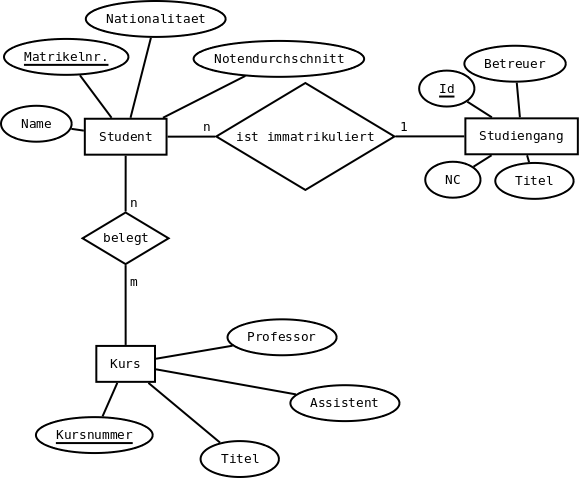
\includegraphics[scale=0.5]{./inc/klausurvorbereitung/klausurvorbereitung.png}
\bigskip

\noindent
$b)$ Bitter "uberf"uhren Sie das soeben erstellte Entity-Relationship-Diagramm in ein Relationenschema.\\


\noindent
\fbox{
    \parbox{\textwidth}{
        Student(\underline{Matrikelnr.}, Name, Nationalitaet, Notendurchschnitt, $\overline{Studiengang}$)\\
        Studiengang(\underline{Id}, Titel, Betreuer, NC)\\
        Kurs(\underline{Kursnummer}, Titel, Professor, Assistent)\\
        Stundenplan(\underline{$\overline{Student}$, $\overline{Kurs}$})
    }
}\\


\noindent
$c)$ Die Struktur ist mittlerweile in einer SQL Datenbank abgelegt.
Der Professor f"ur Algebra m"ochte sich einen "Uberblick "uber die besten Studenten in seinem Kurs machen.
Bitte formulieren Sie folgende SQL Abfrage:\\
Geben Sie alle Studenten mit Namen, Matrikelnummer und Nationalit"at aus, die einen Notendurchschnitt von 1,0 haben und den Kurs Algebra besuchen.
Die Studenten sollen "uber den Namen aufsteigend sortiert werden.

\lstset{style=customSQL}
\begin{lstlisting}
SELECT  s.Name, s.Matrikelnr, s.Nationalitaet
FROM    Student AS s
        , Kurs AS k
        , Stundenplan AS hs
WHERE   s.Matrikelnr = hs.Student
        AND k.Kursnummer = hs.Kurs
        AND s.Notendurchschnitt = 1
        AND k.Titel = 'Algebra'
;
\end{lstlisting}




\section{Mobile Applikationen}

\subsection{Aufgabe 2: Mobile Applikationen}
In der Veranstaltung haben Sie mehrere Arten kennen gelernt, wie mobile Anwendungen umgesetzt werden k"onnen.\\

\noindent
$a)$ nennen Sie zwei serverseitige und zwei clientseitige Technologien die in einer Webanwendung eingesetzt ewrden k"onnen.
\begin{itemize}
    \item Serverseitig
    \begin{itemize}
        \item PHP
        \item asp.NET
    \end{itemize}
    \item Clientseitig
    \begin{itemize}
        \item JavaScript
        \item Flash
        \item Silverlight
        \item JavaApplet
    \end{itemize}
\end{itemize}
\bigskip

\noindent
$b)$ Nennen Sie zwei der am h"aufigsten eingesetzten Betriebssysteme f"ur mobile Ger"ate.\\
\begin{itemize}
    \item Android
    \item iOS
    \item WindowsPhone
\end{itemize}
\bigskip

\noindent
$c)$ Auf mobilen Ger"aten haben Sie zus"atzlich zur Anzeige von Webseiten die M"oglichkeit, native Anwendungen zu entwickeln.
Welche Auswirkung kann dies auf Ihre Technologieentscheidung haben, wenn Sie hardwarefunktionen wie z.B. Video oder Foto verwenden m"ochten?
Nennen Wie mindestens einen Vor- und einen Nachteil von nativen Anwendungen.\\
    Apps die auf Web-Anwendungen basieren k"onnen nicht direkt auf die Hardware des Ger"ates zugreifen.
    Jedoch k"onnen unter zu Hilfe nahme von bestimmten Frameworks so genannte "`hybride Apps"' entwickelt werden, die es erlauben auf plattformspezifische Funktionen und die Hardware des Zielger"ates zu zugreifen.\\
Wenn bei einer zu entwickelnden App bekannt ist, dass in Zukunft Hardwarefunktionen des Ger"ates genutzt werden sollen, ist unbedingt von einer web-basierten L"osung abzuraten.\\
\begin{quote}
    \noindent
    Vor- und Nachteile der nativen Apps:
    \begin{itemize}
        \item Vorteile:
        \begin{itemize}
            \item Zugriff auf die Hardware
            \item Native Apps sind performanter
        \end{itemize}
        \item Nachteile:
        \begin{itemize}
            \item Gro"ser Implementierungsaufwand f"ur Apps, die auf mehreren Plattformen vertrieben werden sollen
        \end{itemize}
    \end{itemize}
\end{quote}
\bigskip

\noindent
$d)$ In der Veranstaltung haben Sie das Konstrukt der User Experience kennen gelenrt.
Bitte beschreiben sie kurz was darunter zu verstehen ist und aus welchen drei Bestandteilen diese zusammengesetzt ist.\\
\begin{quote}
\end{quote}
\bigskip



\section{HTML}

\subsection{Aufgabe 3: HTML}
Der folgende HTML-Code beschreibt vereinfacht eine mobile Webseite:\\
\ldots\\

\noindent
$a)$ Die Webseite enth"alt Fehler, die dem korrekten Aufbau einer HTML-Seite wiedersprechen.
Finden Sie die Fehler und korrigieren Sie diese im Quellcode.

\lstset{style=customXML}
\begin{lstlisting}
<html>
<head>
    <link rel='stylesheet' href='http://serverxy.de/jquery.mobile-1.2.0.min.css'/>
    <script src='http://serverxy.de/jquery-1.8.2.min.js'></script>
    <script src='http://serverxy.de/1.2.0/jquery.mobile-1.2.0.min.js'></script>
</head>
<body>
    <div data-role='page' data-theme='e'>
        <div data-role='header'>
            <h1>APP der FAU</h1>
        </div><!-- /header -->

        <div data-role='content'>
            <img src='http://serverxy.de/Logo.jpg'>
            <ul data-role='listview'>
                <li><a href='http:/serverxy.de/Lehrstuhl1.html'>Lehrstuhl1</a></li>
                <li><a href='http:/serverxy.de/Lehrstuhl2.html'>Lehrstuhl2</a></li>
                <li><a href='http:/serverxy.de/Lehrstuhl3.html'>Lehrstuhl3</a></li>
            </ul>
        </div><!-- /content -->

    </div><!-- /page -->
</body>
</html>
\end{lstlisting}
\bigskip

\noindent
$b)$ Im head der Seite finden Sie drei Elemente.
Welche Funktion haben diese drei Zeilen?\\
\begin{quote}
    Die zus"atzlichen Zeilen sind daf"ur verantwortlich, dass die jQuery-Bibliothek mit dazugeh"origem Style-Sheet geladen werden.
\end{quote}
\bigskip

\noindent
$c)$ Wie ver"andert sich die Seite im Browser nachdem die drei Elemente aufgerufen und ausgef"uhrt wurden?\\
\begin{quote}
    Bei Ausf"uhrung des mobile jQuerys wird erkannt, dass es sich beim Anzeigeger"at um ein "`Mobile Device"' handelt.
    Anschlie"send werden die jQuery betreffenden Attribute der HTML-Tags ausgewertet und umgesetzt.
    Dies betrifft in diesem Fall nur optische "Anderungen.
\end{quote}







